\documentclass[12pt]{article}
\usepackage[pdftex]{color, graphicx}
\usepackage{amsmath, amsfonts, amssymb, mathrsfs}
\usepackage{dcolumn}
\usepackage{natbib}
\usepackage{wrapfig}
\usepackage{subfig}
\usepackage{float}
\bibpunct{(}{)}{;}{a}{}{,}

\oddsidemargin=0.25in
\evensidemargin=0.25in
\textwidth=6in
\textheight=8.75in
\topmargin=-.5in
\footskip=0.5in


\date{due Sep 17th}

\title{Homework3}



\begin{document}

%\maketitle
\newcommand{\argmin}{\text{argmin}}

\noindent STAT5014\\
 Homework 5\\
 Due Oct.1th

\begin{center}
\noindent
\section*{A priliminary study of school aged children's life satisfaction} %this is a comment
\noindent Yin Yuan\\

\vspace{.25 in}
\end{center}

\subsection*{Brief Introduction}

This preliminary study aims to reveal how does the family background factors exert influence on the school aged children's life satisfaction. Global life satisfaction refers to a general evaluation of the quality of a person’s life that is over and above evaluations of specific domains. The life satisfaction of children or youth mirrors their life quality at a certain degree and such early life’s self-rated life evaluation is influential for their current's academic achievement and future career's development. 

Family is the basic unit of society and the essential life source for children. In this study, I attempt to answer a very basic but significant question, how does the family’s socioeconomic status and races factors differentiate the children’s life satisfaction. Socioeconomic status differs by the family wealth and the racial plays a key role for the origins of social inequality. By uncovering the mechanism of how these two factors put effect on children's life satisfaction, I could explore other moderators thereafter.




\subsection*{Data}

1. A berif introduction of the data set\\

This study employs the Health Behavior in School-Aged Children 2009-2010 in U.S. survey data (HBSC 09-10).The U.S. survey is one part of the international HBSC study, which looks at 11-, 13-, and 15-year-old children’s attitudes and experiences concerning a wide range of health-related behaviors and lifestyle issues. It represents a significant opportunity to analyze similarities and differences in health-related behavior for the early- to mid-adolescent age group across the majority of developed countries.

Within the 314 participating schools 14,627 students were found to be eligible to participate. About 2\% of the students refused to consent to the survey. On the day of the survey administration there were 675 students absent. However, a total of 301 of these absent students completed the questionnaire within a couple of days. The final sample size yielded 12,642. This yielded a response rate of just over 90\% of those students who originally consented. \\


2. Basic Demographical characteristics\\

The gender of the HBSC sample is equally distributed as shown by figure (1), with a several points more percentage of boy than girl. In figure (2), we know the number of age ranges from 10 to 17, and the majority is aged from 11 to 15 years old. 

\begin{figure*}[hptb]
	\centering
{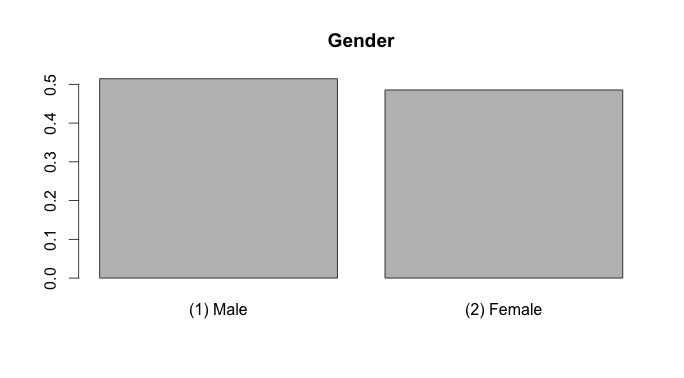
\includegraphics[scale=0.45]{genderpic.png}} \;
\caption{Gender proportion}
	\label{fig:img}
\end{figure*}

\begin{figure*}[hptb]
	\centering
{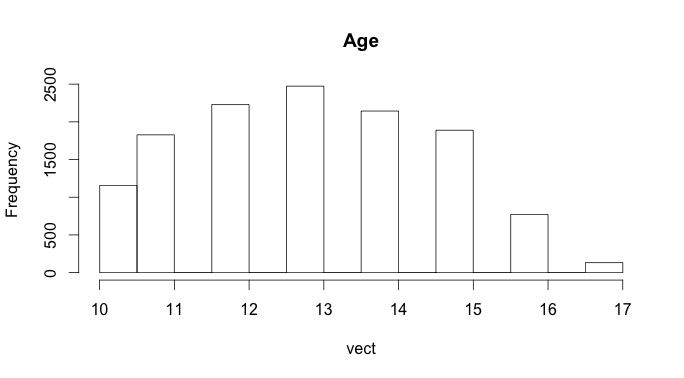
\includegraphics[scale=0.45]{agepic.png}} \;
\caption{Age}
	\label{fig:img}
\end{figure*}

3. Variables
Depenent variable: life satisfaction

Independent variable: races,   family affluence



\subsection*{Appendix: R code}
\begin{verbatim}
load("~/Documents/STAT5014/hw5/ICPSR_34792/DS0001/HBS.rda")

#barchar and histgram description for basic demographical characteristics, gender and age:

plotfuncthw5=function(vect, title){
  if(is.numeric(vect)) {
    hist(vect, main=title)
  }
  else {
    frequency <- table(vect)
    prop <- frequency/sum(frequency)
    #print(prop)
    barplot(prop, main=title)
  }
 }

plotfuncthw5(Q1,"Gender")

plotfuncthw5(Q3B,"Age")

#boxplot drawing:

for( i in 1:length(unique(Q6_COMP))){
                                    assign(paste0("data",i),subset(da34792.0001,
                                    Q6_COMP==unique(Q6_COMP)[i]))
}

data<-list(data2,data3,data4,data5,data6,data7,data8)

for( i in 2:8){
               J<-unique(Q6_COMP)[i]
               plot(get(paste0("data",i))$Q11,get(paste0("data",i))$Q7,xlab="Family        
               Affluence",ylab="Life Satisfaction",
               main=paste("Life Satisfaction by Family 
               Affluence"),sub=strsplit(as.character(J),")")[[1]][2])
}
\end{verbatim}

\begin{figure*}[hptb]
	\centering
{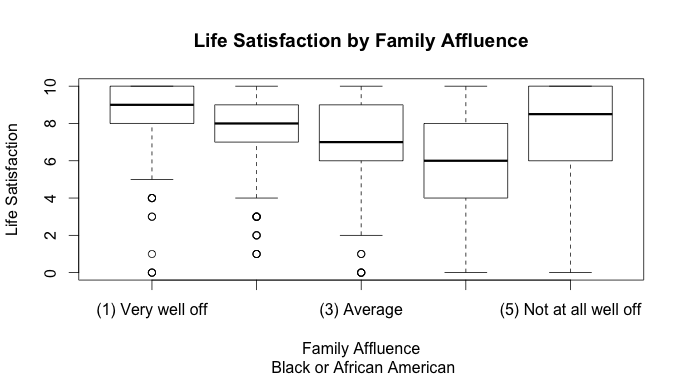
\includegraphics[scale=0.45]{boxplotafrican.png}} \;
\caption{......}
	\label{fig:img}
\end{figure*}

\begin{figure*}[hptb]
	\centering
{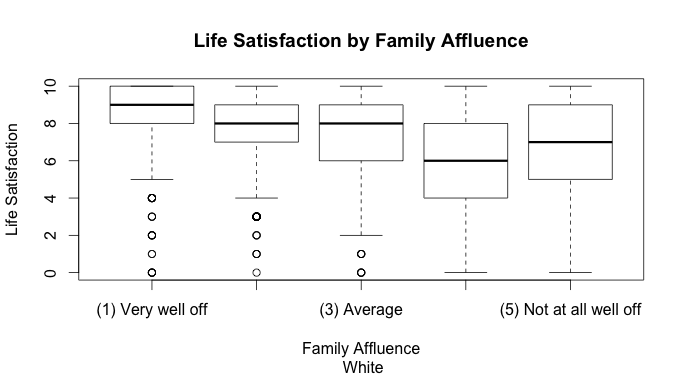
\includegraphics[scale=0.45]{boxplotwhite.png}} \;
\caption{.......}
	\label{fig:img}
\end{figure*}

\begin{figure*}[hptb]
	\centering
{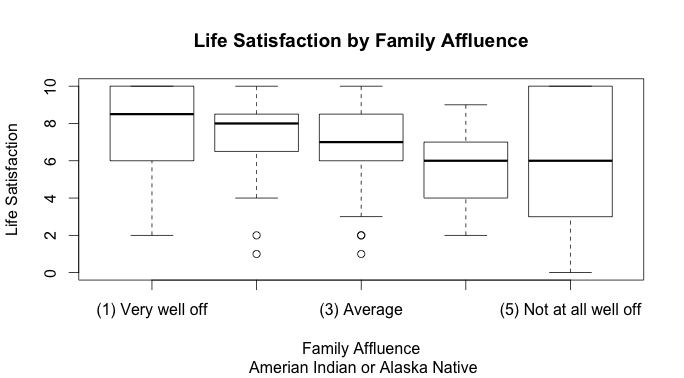
\includegraphics[scale=0.45]{boxplotamericanindian.png}} \;
\caption{.......}
	\label{fig:img}
\end{figure*}

\begin{figure*}[hptb]
	\centering
{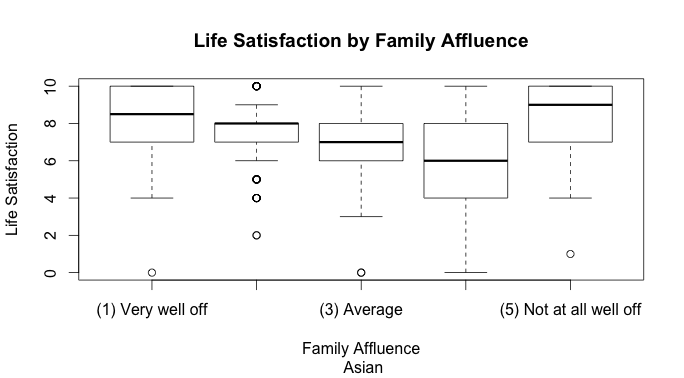
\includegraphics[scale=0.45]{boxplotasian.png}} \;
\caption{.......}
	\label{fig:img}
\end{figure*}

\begin{figure*}[hptb]
	\centering
{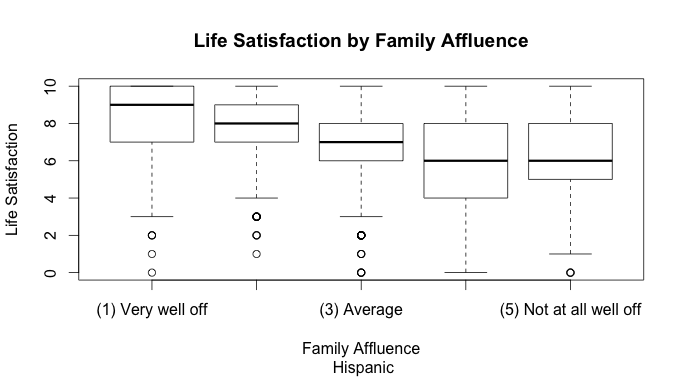
\includegraphics[scale=0.45]{boxplothispanic.png}} \;
\caption{.......}
	\label{fig:img}
\end{figure*}

\begin{figure*}[hptb]
	\centering
{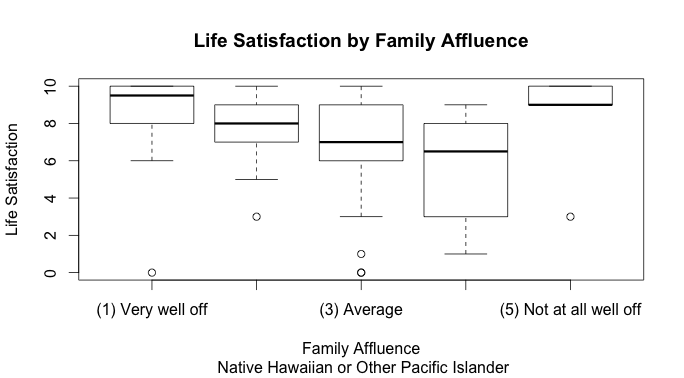
\includegraphics[scale=0.45]{boxplotislander.png}} \;
\caption{.......}
	\label{fig:img}
\end{figure*}

\begin{figure*}[hptb]
	\centering
{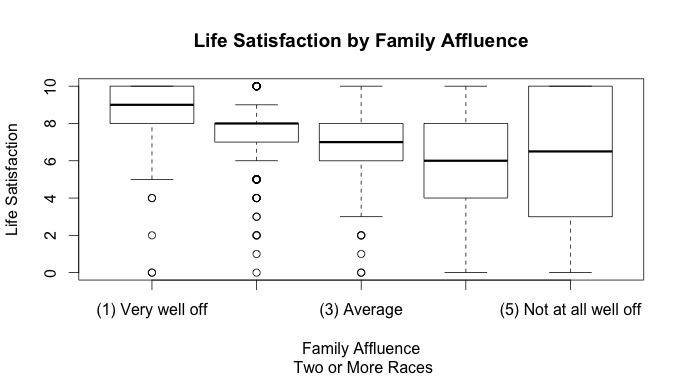
\includegraphics[scale=0.45]{boxplotmoreraces.png}} \;
\caption{.......}
	\label{fig:img}
\end{figure*}




\end{document}



